\documentclass[cal1spr16Lectures.tex]{subfiles}

\begin{document}

\section[Week 8]{Week 8: 7-11 Mar}

% % %
\subsection{Midterm Review}
% % %

% % %
\begin{frame}[allowframebreaks]{Midterm Review}\footnotesize
\begin{itemize}
\item \S 2.1-2.2 
	\begin{itemize}\footnotesize
	\item {\bf Material may not be explicitly tested, but the topics here are foundational to later sections.}
	\end{itemize}
%\framebreak	
\item \S 2.3 Techniques for Computing Limits
	\begin{itemize}\footnotesize
	\item {\bf Be able to do questions similar to 1-48.}
	\item Know and be able to compute limits using analytical methods (e.g., limit laws, additional techniques).
	\item Be able to evaluate one-sided and two-sided limits of functions.
	\item Know the Squeeze Theorem and be able to use this theorem to determine limits.
	\end{itemize}
\framebreak
\begin{exe}[problems from past midterm] Evaluate the following limits:
\begin{itemize}
\item $\displaystyle\lim_{x\to 3}\frac{x^2-x-6}{x^2-9}$
\item $\displaystyle\lim_{\theta\to 0}\frac{\sec\theta\tan\theta}{\theta}$
\end{itemize}
\end{exe}
%
\framebreak
\item \S 2.4 Infinite Limits
	\begin{itemize}\footnotesize
	\item {\bf Be able to do questions similar to 17-30.}
	\item Be able to use a graph, a table, or analytical methods to determine infinite limits.
	\item Be able to use analytical methods to evaluate one-sided limits.
	\item Know the \alert{definition} of a vertical asymptote and be able to determine whether a function has vertical asymptotes.
	\end{itemize}
%
\framebreak
\item \S 2.5 Limits at Infinity
	\begin{itemize}\footnotesize
	\item {\bf Be able to do questions similar to 9-30 and 38-46.}
	\item Be able to find limits at infinity and horizontal asymptotes. 
	\item Know how to compute the limits at infinity of rational functions and algebraic functions.
	\item Be able to list horizontal and/or vertical asymptotes of a function.
	\end{itemize}
\begin{exe}
Determine the horizontal asymptote(s) for the function
\[
f(x)=\frac{10x^3-3x^2+8}{\sqrt{25x^6+x^4+2}}
\]
\begin{itemize}
\item[A. ] $y=2$
\item[B. ] $y=0$
\item[C. ] $y=-2$
\item[D. ] $y=\pm 2$
\end{itemize}
\end{exe}	

\framebreak	
\item \S 2.6 Continuity
	\begin{itemize}\footnotesize
	\item {\bf Be able to do questions similar to 9-44.}
	\item Know the definition of continuity and be able to apply the continuity checklist.
	\item Be able to determine the continuity of a function (including those with roots) on an interval.
	\item Be able to apply the Intermediate Value Theorem to a function.
	\end{itemize}
\framebreak
\begin{exe}[problem from past midterm]
Determine the value of $k$ so the function is continuous on $0\leq x\leq 2$.
\[f(x)=\begin{cases}x^2+k & 0\leq x\leq 1 \\
	-2kx+4 & 1<x\leq 2\end{cases}
	\]
\end{exe}	

\framebreak
\item \S 3.1 Introducing the Derivative
	\begin{itemize}\footnotesize
	\item {\bf Be able to do questions similar to 11-32.}
	\item Know the definition of a derivative and be able to use this definition to calculate the derivative of a given function.
	\item Be able to determine the equation of a line tangent to the graph of a function at a given point.
	\item Know the 3 conditions for when a function is not differentiable at a point, and why these three conditions make a function not differentiable at the given point.
	\end{itemize}

\framebreak
\item \S 3.2 Working with Derivatives
	\begin{itemize}\footnotesize
	\item Be able to use the graph of a function to sketch the graph of its derivative, without computing derivatives
	\item Know the 3 conditions for when a function is not differentiable at a point, and why these three conditions make a function not differentiable at the given point
	\item Be able to determine where a function is not differentiable
	\end{itemize}
%
\framebreak	
\item \S 3.3 Rules for Differentiation
	\begin{itemize}\footnotesize
	\item {\bf Be able to do questions similar to 7-41.}
	\item Be able to use the various rules for differentiation (e.g., constant rule, power rule, constant multiple rule, sum and difference rule) to calculate the derivative of a function.
	\item Know the derivative of $e^x$.
	\item Be able to find slopes and/or equations of tangent lines.
	\item Be able to calculate higher-order derivatives of functions.
	\end{itemize}
%
\framebreak
\begin{exe}
Given that $y=3x+2$ is tangent to $f(x)$ at $x=1$ and that $y=-5x+6$ is tangent to $g(x)$ at $x=1$, write the equation of the tangent line to $h(x)=f(x)g(x)$ at $x=1$.
\end{exe}
%
\framebreak
\item \S 3.4 The Product and Quotient Rules
	\begin{itemize}\footnotesize
	\item {\bf Be able to do questions similar to 7-42 and 47-52.}
	\item Be able to use the product and/or quotient rules to calculate the derivative of a given function.
	\item Be able to use the product and/or quotient rules to find tangent lines and/or slopes at a given point.
	\item Know the derivative of $e^{kx}$.
	\item Be able to combine derivative rules to calculate the derivative of a function.
	\end{itemize}
	
{\bf Note:} Functions are not always given by a formula.  When faced with a problem where you don't know where to start, go through the rules first.
%
\framebreak
\begin{exe} Suppose you have the following information about the functions $f$ and $g$:
\[f(1)=6\quad f'(1)=2\quad g(1)=2\quad g'(1)=3\]
\vspace{-1pc}	
	\begin{itemize}\footnotesize
	\item Let $F=2f+3g$.  What is $F(1)$?  What is $F'(1)$?
	\item Let $G=fg$.  What is $G(1)$?  What is $G'(1)$?
	\end{itemize}
\end{exe}
%
\framebreak
\item \S 3.5 Derivatives of Trigonometric Functions
	%\vspace{-0.75pc}
	\begin{itemize}\footnotesize
	\item {\bf Be able to do questions similar to 1-55.}
	\item Know the two special trigonometric limits
	\vspace{-0.5pc}
	\[\lim_{x\to 0}\frac{\sin x}{x}=1\qquad\text{and}\qquad\lim_{x\to 0}\frac{\cos x-1}{x}=0\]
	and be able to use them to solve other similar limits.
	\item Know the derivatives of $\sin x$, $\cos x$, $\tan x$, $\cot x$, $\sec x$, $\csc x$, and be able to use the quotient rule to derive the derivatives of $\tan x$, $\cot x$, $\sec x$, and $\csc x$.
	\item Be able to calculate derivatives (including higher order) involving trig functions using the rules for differentiation.
	\end{itemize}
%
\framebreak
\begin{exe}
Calculate the derivative of the following functions:
\begin{itemize}
\item $f(x)=(1+\sec x)\sin^3x$
%
%\vspace{1pc}
\item $g(x)=\displaystyle\frac{\sin x+\cot x}{\cos x}$
\end{itemize}
\end{exe}
%
%
\begin{exe} Evaluate $\displaystyle\lim_{x\to -3}\frac{\sin{(x+3)}}{x^2+8x+15}$. \end{exe}
%
%
\framebreak
\item \S 3.6 Derivatives as Rates of Change
	\begin{itemize}\footnotesize
	\item {\bf Be able to do questions similar to 11-18.}
	\item Be able to use the derivative to answer questions about rates of change involving:
		\begin{itemize}%\tiny
		\item Position and velocity
		\item Speed and acceleration
		\item Growth rates
		\item Business applications
		\end{itemize}
\framebreak		
	\item Be able to use a position function to answer questions involving velocity, speed, acceleration, height/distance at a particular time $t$, maximum height, and time at which a given height/distance is achieved.
	\item Be able to use growth models to answer questions involving growth rate and average growth rate, and cost functions to answer questions involving average and marginal costs.
	\end{itemize}
%
\framebreak
\item \S 3.7 The Chain Rule
	\begin{itemize}\footnotesize
	\item {\bf Be able to do questions similar to 7-43.}
	\item Be able to use both versions of the Chain Rule to find the derivative of a composition function.
	\item Be able to use the Chain Rule more than once in a calculation involving more than two composed functions.
	\item Know and be able to use the Chain Rule for Powers:
	\[\frac{d}{dx}\left(f(x)\right)^n=n\left(f(x)\right)^{n-1}f'(x)\]
	\end{itemize}
\framebreak
\begin{exe} Suppose $f'(9)=10$ and $g(x)=f(x^2)$.  What is $g'(3)$? \end{exe}
%
\framebreak
\item \S 3.8 Implicit Differentiation
	\begin{itemize}\footnotesize
	\item {\bf Be able to do questions similar to 5-26 and 33-46.}
	\item Be able to use implicit differentiation to calculate $\textstyle\frac{dy}{dx}.$
	\item Be able to use the derivative found from implicit differentiation to find the slope at a given point and/or a line tangent to the curve at the given point.
	\item Be able to calculate higher-order derivatives of implicitly defined functions.
	\item Be able to calculate $\textstyle\frac{dy}{dx}$ when working with functions containing rational functions.
	\end{itemize}
%
\begin{exe} Use implicit differentiation to calculate $\textstyle\frac{dz}{dw}$ for
\[e^{2w}=\sin(wz)\]
\end{exe}
\begin{exe} If $\sin x=\sin y$, then 
\begin{itemize}\footnotesize
\item $\textstyle\frac{dy}{dx}=$ ? 
\item $\textstyle\frac{d^2y}{dx^2}=$ ? 
\end{itemize}
\end{exe}
\framebreak
\item \S 3.9 Derivatives of Logarithmic and Exponential Functions
	\vspace{-0.5pc}
	\begin{itemize}\footnotesize
	\item Be able to compute derivatives involving $\ln x$ and $\log_b x$
	\item Be able to compute derivatives of exponential functions of the form $b^x$
	\item Be able to use logarithmic differentiation to determine $f^{\prime}(x)$
	\end{itemize}

\end{itemize}
\end{frame}

% % % 
\subsubsection{Running Out of Time on the Exam Plus other Study Tips}
% % %
\begin{frame}[allowframebreaks]{\small Running Out of Time on the Exam Plus other Study Tips}\footnotesize
\begin{itemize}
\item Do practice problems completely, from beginning to end (as if it were a quiz).  You might think you understand something but when it's time to write down the details things are not so clear.  
\item Find a buddy who understands concepts a little better than you and work on problems for 2-3 hours.  Then find a buddy who is struggling and work with them 2-3 hours.  %Explaining to someone else tests how deeply you really know the material.  This strategy also helps reduce stress because it doesn't require you to devote a full day or night of studying, just 2-3 hours at a time of productive work.
\item Don't count on cookie cutter problems.  If you are doing a practice problem where you've memorized all the steps, make sure you understand why each step is needed.  The exam problems may have a small variation from homeworks and quizzes.  If you're not prepared, it'll come as a ``twist" on the exam...
%
\framebreak
\item If you encounter an unfamiliar type of problem on the exam, relax, because it's most likely not a trick!  The solutions will always rely on the information from the required reading/assignments.  Take your time and do each baby step carefully.  
\item During the exam, do the problems you are most confident with first!  %Different people will find different problems easier.
\item During the exam, budget your time.  Count the problems and divide by 50 minutes.  The easier questions will take less time so doing them first leaves extra time for the harder ones.  When studying, aim for 10 problems per hour (i.e., 6 minutes per problem).
%
\framebreak
\item Always make sure you \alert{answer the question}.  This is also a good strategy if you're not sure how to start a problem, figure out what the question wants first.
\item The exam is not a race.  If you finish early take advantage of the time to check your work.  You don't want to leave feeling smug about how quickly you finished only to find out next week you lost a letter grade's worth of points from silly mistakes.
\end{itemize}
\end{frame}

% % %
\subsubsection{Other Study Tips}
% % %

% % %
\begin{frame}{\small Other Study Tips}
\footnotesize
\begin{itemize}
\item Brush up on algebra, especially radicals, logs, common denominators, etc.  Many times knowing the right algebra will simplify the problem!
\item When in doubt, show steps.  
\item You will be punished for wrong notation.  The slides for \S 3.1 show different notations for the derivative.  Make sure whichever one you use in your work, that you are using it correctly.
\item Read the question!  
\item Do the book problems.
\item Look at the pictures in the book and the interactive applets on MLP.
\end{itemize}
\end{frame}

% % %
\subsection[3.10 Derivatives of Inverse Trigonometric Functions]{\S 3.10 Derivatives of Inverse Trigonometric Functions}
% % %

% % %
\begin{frame}{\S 3.10 Derivatives of Inverse Trigonometric Functions}{}\small
{\bf Recall:} If $y=f(x)$, then $f^{-1}(x)$ is the value of $y$ such that $x=f(y)$.
\begin{ex} If $f(x)=3x+2$, then what is $f^{-1}(x)$? \end{ex}
{\bf NOTE:}  $f^{-1}(x)\alert{\neq} f(x)^{-1}\textstyle\left(=\frac{1}{f(x)}\right)$

\vspace{0.5pc}
To avoid this confusion, we use $\arcsin{x},\,\arccos{x}\,\arctan{x},\dots$ to denote inverse trig functions.
\end{frame}

% % %
\subsubsection{Derivative of Inverse Sine}
% % %

% % %
\begin{frame}{\small Derivative of Inverse Sine}
Trig functions are functions, too.  Just like with ``$f\,$", there has to be something to ``plug in".  It makes no sense to just say $\sin$, without having $\sin(\text{\alert{\it something}})$.
\[y=\sin^{-1}x \Longleftrightarrow x=\sin y\]  
\end{frame}

% % %
\begin{frame}\footnotesize
The derivative of $y=\sin^{-1}x$ can be found using implicit differentiation: 
\begin{alignat*}{2}
x &= \sin y \\
\frac{d}{dx}(x) &= \frac{d}{dx}(\sin y) \\
1 &= (\cos y) \frac{dy}{dx} \\
\frac{dy}{dx} &= \frac{1}{\cos y}
\end{alignat*}
\end{frame}

% % %
\begin{frame}\footnotesize
We still need to replace $\cos y$ with an expression in terms of $x$.  We use the trig identity $\sin^2 y + \cos^2 y = 1$ (careful with notation: in this case we mean $\left(\sin y\right)^2+\left(\cos y\right)^2=1$).  Then 
\[\cos y= \pm \sqrt{1-\sin^2 y}=\pm\sqrt{1-x^2}.\]
The range of $y=\sin^{-1}x$ is $-\textstyle\frac{\pi}{2} \leq y \leq \frac{\pi}{2}$.  In this range, cosine is never negative, so we can just take the positive portion of the square root.
Therefore,
\[\frac{dy}{dx}=\frac{1}{\cos y}=\frac{1}{\sqrt{1-x^2}} \implies \alert{\frac{d}{dx}(\sin^{-1}x)=\frac{1}{\sqrt{1-x^2}}}.\]
\end{frame}

% % %
\begin{frame}{}
\begin{exe} Compute the following:
\begin{itemize}
\item[1.] $\frac{d}{dx} \left( \sin^{-1}(4x^2-3) \right)$
\item[2.] $\frac{d}{dx} \left( \cos(\sin^{-1}x) \right)$
\end{itemize}
\end{exe}
\end{frame}

% % %
\subsubsection{Derivative of Inverse Tangent}
% % %

% % %
\begin{frame}{\small Derivative of Inverse Tangent}\footnotesize
Similarly to inverse sine, we can let $y=\tan^{-1}x$ and use implicit differentiation:
\vspace{-0.5pc}
\begin{alignat*}{2}
x &= \tan y \\
\frac{d}{dx}(x) &= \frac{d}{dx} (\tan y) \\
1 &= (\sec^2 y) \frac{dy}{dx} \\
\frac{dy}{dx} &= \frac{1}{\sec^2 y}
\end{alignat*}
\end{frame}

% % %
\begin{frame}
Use the trig identity $\sec^2 y-\alert{\tan^2 y}=1$ to replace $\sec^2 y$ with $1+\alert{x^2}$:
\[\alert{\frac{d}{dx}(\tan^{-1} x)=\frac{1}{1+x^2}}\]
\end{frame}

% % %
\subsubsection{Derivative of Inverse Secant}
% % %

% % %
\begin{frame}{\small Derivative of Inverse Secant}\footnotesize
Again, use the same method as with inverse sine:
\begin{alignat*}{2}
y &= \sec^{-1}x \\
x &= \sec y \\
\frac{d}{dx}(x) &= \frac{d}{dx} (\sec y) \\
1 &= \sec y \tan y \frac{dy}{dx} \\
\frac{dy}{dx} &= \frac{1}{\sec y \tan y}
\end{alignat*}
\end{frame}

% % %
\begin{frame}\footnotesize
Use the trig identity $\sec^2 y-\tan^2 y=1$ again to get 
\[\tan y=\pm\sqrt{\sec^2 y-1}=\pm\sqrt{x^2-1}.\]
This time, the $\pm$ matters:
\vspace{-1.1pc}
\begin{columns}
\begin{column}{0.3\textwidth}
	\begin{center}\includegraphics[scale=0.49]{pictures/invSecpic}\end{center}
\end{column}
\begin{column}{0.6\textwidth}
	\begin{itemize}
	\item If $x \ge 1$, then $0\leq y<\textstyle\frac{\pi}{2}$ and so $\tan y >0.$  
	\item If $x \le -1$, then $\textstyle\frac{\pi}{2} < y \leq \pi$ and so  $\tan y <0$.  
	\end{itemize}
\end{column}
\end{columns}	
\end{frame}

% % %
\begin{frame}\footnotesize
Therefore,
\[\alert{\frac{d}{dx}(\sec^{-1} x)=\frac{1}{|x|\sqrt{x^2-1}}}.\]
\hrulefill

Using other trig identities (which you do not need to prove)
\[\cos^{-1}x+\sin^{-1}x=\frac{\pi}{2}\quad \cot^{-1}x+\tan^{-1}x=\frac{\pi}{2}\quad \csc^{-1}x+\sec^{-1}x=\frac{\pi}{2}\] 
we can get the rest of the inverse trig derivatives. 
\end{frame}

% % %
\subsubsection{All Other Inverse Trig Derivatives}
% % %

% % %
\begin{frame}{\small All Other Inverse Trig Derivatives}
To summarize:
\begin{columns}
\begin{column}{0.45\textwidth}
	\begin{itemize}
	\item[]$\textstyle\frac{d}{dx}(\sin^{-1}x)=\frac{1}{\sqrt{1-x^2}}$
	\item[]$\textstyle\frac{d}{dx}(\tan^{-1}x)=\frac{1}{1+x^2}$ 
	\item[]$\textstyle\frac{d}{dx}(\sec^{-1}x)=\frac{1}{|x|\sqrt{x^2-1}}$ 
	\end{itemize}
\end{column}
\begin{column}{0.6\textwidth}
	\begin{itemize}
	\item[] \alert{$\textstyle\frac{d}{dx}(\cos^{-1}x)=-\frac{1}{\sqrt{1-x^2}}$} \\
	$\quad (-1<x<1)$ 
	\item[] \alert{$\textstyle\frac{d}{dx}(\cot^{-1}x)=-\frac{1}{1+x^2}$} \\
	$\quad (-\infty<x<\infty) $ 
	\item[] \alert{$\textstyle\frac{d}{dx}(\csc^{-1}x)=-\frac{1}{|x|\sqrt{x^2-1}}$} \\
	$\quad (|x|>1)$ 
	\end{itemize}
\end{column}
\end{columns}
\end{frame}

% % %
\begin{frame}
\begin{ex} Compute the derivatives of $f(x)=\tan^{-1}\left(\textstyle\frac{1}{x}\right)$ and $g(x)=\sin \left(\sec^{-1}(2x) \right)$. \end{ex}
\end{frame}

% % %
\subsubsection{Derivatives of Inverse Functions in General}
% % %

% % %
\begin{frame}{\small Derivatives of Inverse Functions in General}\footnotesize
Let $f$ be differentiable and have an inverse on an interval $I$.  Let $x_0$ be a point in $I$ at which $f^{\prime}(x_0)\ne0$.  Then $f^{-1}$ is differentiable at $y_0=f(x_0)$ and 
\[\left(f^{-1}\right)^{\prime}(y_0)=\frac{1}{f^{\prime}(x_0)}\]
where $y_0=f(x_0)$.
\begin{ex} Let $f(x)=3x+4$.  Find $f^{-1}(x)$ and $\left(f^{-1}\right)^{\prime}\left(\textstyle\frac{1}{3}\right)$. \end{ex}
\end{frame}

% % %
\subsubsection{Book Problems}
% % %

% % %
\begin{frame}
\begin{block}{3.10 Book Problems} 7-33 (odds), 37-41 (odds) \end{block}
\end{frame}

% % %
\subsection[3.11 Related Rates]{\S 3.11 Related Rates}
% % %

% % %
\begin{frame}{\S 3.11 Related Rates}
\small 
In this section, we use our knowledge of derivatives to examine how variables change with respect to time.

\vspace{1pc}
The prime feature of these problems is that two or more variables, which are related in a known way, are themselves changing in time.

\vspace{1pc}
The goal of these types of problems is to determine the rate of change (i.e., the derivative) of one or more variables at a specific moment in time.
\end{frame}

% % %
\begin{frame}
\frametitle{}
\begin{block}{Problem}
The edges of a cube increase at a rate of 2 cm/sec.  How fast is the volume changing when the length of each edge is 50 cm?
\end{block}
\small
\begin{itemize}
\item {\bf Variables:}  $V$ (Volume of the cube) and $x$ (length of edge)
\item {\bf How Variables are related:}  $V=x^3$
\item {\bf Rates Known:}  $\dfrac{dx}{dt}=2\ \text{cm/sec}$
\item {\bf Rate We Seek:}  $\dfrac{dV}{dt}$ when $x=50\ \text{cm}$
\end{itemize}
\end{frame}

% % % 
\begin{frame}
\small
Note that both $V$ and $x$ are functions of $t$ (their respective sizes are dependent upon how much time has passed).

\vspace{1pc}
So we can write $V(t)=x(t)^3$ and then differentiate this with respect to $t$:
$$V^{\prime}(t) = 3 x(t)^2 \cdot x^{\prime}(t).$$

\vspace{1pc}
{\bf Note that $x(t)$ is the length of the cube's edges at time $t$, and $x^{\prime}(t)$ is the rate at which the edges are changing at time $t$.}
\end{frame}

% % %
\begin{frame}

We can rewrite the previous equation as

\[\frac{dV}{dt}=3x^2 \cdot \frac{dx}{dt}.\]

\vspace{1pc}
So the rate of change of the volume when $x=50\ \text{cm}$ is 
\[\left.\frac{dV}{dt}\right|_{x=50}=3\cdot 50^2 \cdot 2 = 15000\ \text{cm}^3/\text{sec}.\]
\end{frame}

% % %
\subsubsection{Steps for Solving Related Rates Problems}
% % % 

% % %
\begin{frame}{\small Steps for Solving Related Rates Problems}
\small
\begin{itemize}
\item[1.] Read the problem carefully, making a sketch to organize the given information.  Identify the rates that are given and the rate that is to be determined.
\item[2.] Write one or more equations that express the basic relationships among the variables.
\item[3.] Introduce rates of change by differentiating the appropriate equation(s) with respect to time $t$.
\item[4.] Substitute known values and solve for the desired quantity.
\item[5.] Check that the units are consistent and the answer is reasonable.
\end{itemize}
\end{frame}

% % %
\begin{frame}
\frametitle{}
\begin{block}{The Jet Problem}
A jet ascends at a $10^{\circ}$ angle from the horizontal with an airspeed of 550 miles/hr (its speed along its line of flight is 550 miles/hr).  How fast is the altitude of the jet increasing?  If the sun is directly overhead, how fast is the shadow of the jet moving on the ground?
\end{block}
\end{frame}

% % %
\begin{frame}
\small
{\bf Step 1:}  There are three variables:  the distance the shadow has traveled ($x$), the altitude of the jet ($h$), and the distance the jet has actually traveled on its line of flight ($z$).  We know that $\textstyle\frac{dz}{dt}=550\ \text{miles/hr}$ and we want to find $\textstyle\frac{dx}{dt}$ and $\textstyle\frac{dh}{dt}$.  We also see that these variables are related through a right triangle:
\begin{center}
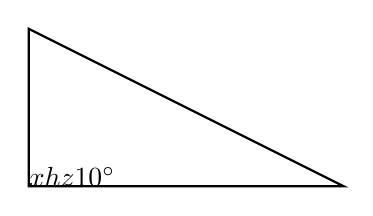
\begin{tikzpicture}[thick]
\coordinate (O) at (0,0);
\coordinate (A) at (4,0);
\coordinate (B) at (0,2);
\draw (O)--(A)--(B)--cycle;
\tkzLabelSegment[below=2pt](O,A){$x$}
\tkzLabelSegment[left=2pt](O,B){$h$}
\tkzLabelSegment[above right=2pt](A,B){$z$}
%\tkzMarkAngle[fill= orange,size=0.65cm,opacity=.4](A,O,B)
%\tkzLabelAngle[pos = 0.35](A,O,B){$\gamma$}
\tkzMarkAngle[size=0.7cm,opacity=.4](B,A,O)
\tkzLabelAngle[pos = 1.3](B,A,O){$10^{\circ}$}
%\tkzMarkAngle[fill= orange,size=0.7cm,opacity=.4](O,B,A)
%\tkzLabelAngle[pos = 0.5](O,B,A){$\beta$}
\end{tikzpicture}
\end{center}
\end{frame}

% % %
\begin{frame}
\small
{\bf Step 2:}  To answer how fast the altitude is increasing, we need an equation involving only $h$ and $z$.  Using trigonometry,
\[\sin(10^{\circ})=\frac{h}{z} \implies h=\sin(10^{\circ}) \cdot z.\]

\vspace{1pc}
To answer how fast the shadow is moving, we need an equation involving only $x$ and $z$.  Using trigonometry,
\[\cos(10^{\circ})=\frac{x}{z} \implies x=\cos(10^{\circ}) \cdot z.\]
\end{frame}

% % %
\begin{frame}
\footnotesize
{\bf Step 3:}  We can now differentiate each equation to answer each question:
\begin{alignat*}{2}
h=\sin(10^{\circ}) \cdot z &\implies \dfrac{dh}{dt}=\sin(10^{\circ}) \dfrac{dz}{dt} \\
x=\cos(10^{\circ}) \cdot z &\implies \dfrac{dx}{dt}=\cos(10^{\circ}) \dfrac{dz}{dt}
\end{alignat*}

\vspace{1pc}
{\bf Step 4:}  We know that $\textstyle\frac{dz}{dt}=550\ \text{miles/hr}$.  So 
\begin{alignat*}{2}
\dfrac{dh}{dt} &=\sin(10^{\circ}) \cdot 550 \approx 95.5\ \text{miles/hr}\\
\dfrac{dx}{dt} &=\cos(10^{\circ}) \cdot 550 \approx 541.6\ \text{miles/hr}
\end{alignat*}
\end{frame}

% % %
\begin{frame}
\frametitle{}
{\bf Step 5:}  Because both answers are in terms of miles/hr and both answers seem reasonable within the context of the problem, we conclude that the jet is gaining altitude at a rate of 95.5 miles/hr, while the shadow on the ground is moving at about 541.6 miles/hr.
\end{frame}

% % %
\begin{frame}\small
\begin{ex} The sides of a cube increase at a rate of $R$ cm/sec.  When the sides have a length of 2 cm, what is the rate of change of the volume? \end{ex}

\begin{ex} Two boats leave a dock at the same time.  One boat travels south at 30 miles/hr and the other travels east at 40 miles/hr.  After half an hour, how fast is the distance between the boats increasing? \end{ex}
\end{frame}

% % %
\begin{frame}
\begin{exe}
A 13 foot ladder is leaning against a vertical wall when Jack begins pulling the foot of the ladder away from the wall at a rate of 0.5 ft/sec.  How fast is the top of the ladder sliding down the wall when the foot of the ladder is 5 ft from the wall?
\end{exe}
\end{frame}

% % % 
\subsubsection{Book Problems}
% % % 

% % %
\begin{frame}
\begin{block}{3.11 Book Problems}
5-14, 16-19, 21-24, 37-38
\end{block}
\end{frame}

\end{document}